\section{Types for Nondeterminism\label{sec:approach}}
%\begin{figure}
%    \begin{center}
%        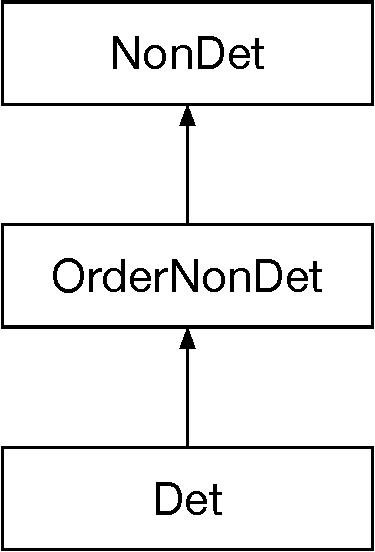
\includegraphics[scale=0.37]{detHierarchy}
%    \end{center}
%    \caption{Determinism type qualifier hierarchy}
%    \label{fig:determinism-hierarchy}
%\end{figure}

We defined a type system
that allows programmers to express (non)determinism properties.
The most novel part of our analysis is how it handles collections that will
contain the same values, but
possibly in a different order, on different runs.


%\todo{This is the first mention of
%    the determinism type system, and the first mention of types since the
%    abstract.  This is sudden and unexpected, and it will confuse readers.
%    You need to say that you will take this approach to solving the problem!}
%\todo{The introduction of the type
%    qualifiers is too sudden, too.  What are type qualifiers?  How are they
%    used?  Why does a reader care?  You should say that every expression in
%    the program is classified as one of the following categories.}

A type abstracts or restricts the set of possible
run-time values that an expression may evaluate to and the operations that
may be performed on it.
A programming language provides \emph{basetypes}, such as \<Int>.
A \textit{type qualifier} on a basetype adds additional constraints;
that is, it reduces the size of the set of values.
An example type qualifier is \<Positive>, and a type (which combines a qualifier
and a basetype) is \<Positive Int>.

The core of the determinism type system
is the following type qualifiers:
\begin{itemize}
    \item \<NonDet> indicates
    that the expression might have different values in two different executions.
    \item \<OrderNonDet> indicates that the expression is a collection or
    a map that contains the same elements in every execution, but possibly
    in a different order.
    \item \<Det> indicates that the expression evaluates to equal values in
    all executions; for a collection, iteration
    also yields the values in the same order.
\end{itemize}
% Every expression in a program is classified as either \<NonDet>, \<OrderNonDet>, or \<Det>.
%\todo{In a \LaTeX\ paper, use the standard mathematical symbols, not ASCII
%  approximations to them.}
The subtyping relationship among the type qualifiers is \<Det> $\sqsubseteq$ \<OrderNonDet> $\sqsubseteq$ \<NonDet>.
%\Cref{fig:determinism-hierarchy} shows the subtyping
%relationship among the qualifiers.
% Programmers can write these type qualifiers to specify their program's behavior. 
The following code is an example of a valid program that type checks. 
%\todo{This code is in poor style.  It assigns to a formal parameter, which
%  is unusual, it performs computation that is ignored (because its return
%  type is void).  Always make your examples as realistic as possible.  One
%  reason is that the code will be easier to read and less surprising or
%  distracting to readers.  Another reason is that if your code is
%  unrealistic, then readers will get the impression that your system is
%  impractical (because you couldn't think of a single real-world
%  application).  Make this code more realistic, or even use an example from
%  one of the libraries or programs.}
\begin{Verbatim}
public class Accesses {
    public NonDet int field1;
    public NonDet int field2;
        void setFields(NonDet int arg1, 
        Det int arg2) {
            field1 = arg1;
            field2 = arg2;
    }
}
\end{Verbatim}
%\todo{The use of ``type'' is confusing.  The paper improperly uses it for
%  qualifiers and return values.  Use the proper term.  When talking about a
%  type, use a type as you just defined it, not just a qualifier.}
All the assignments in this program 
satisfy the subtyping relationships.
 
The following method (From Junit~\cite{junit}), however, doesn't type check.
\begin{Verbatim}
public static Det Method Det[] getDeclaredMethods(
Class<?> clazz) {
    // Error: assignment type incompatible
    Det Method Det[] methods = 
    clazz.getDeclaredMethods();
    ...
    // Error: return type incompatible
    return methods;
}
\end{Verbatim}
The declared return type is annotated as \codeid{Det Method Det[]} (i.e a \<Det> array of \<Det Method> elements).
The call to \<getDeclaredMethods()> returns an array of type \codeid{Det Method OrderNonDet[]}
causing \theDeterminismChecker to issue a warning.
Note that \<getDeclaredMethods()> is a method in the JDK that provides no guarantees on the order of
the elements in the array that it returns and therefore we annotated its return type
as an \<OrderNonDet> array.
%\todo{``The return type is not a subtype of the return type'' does not make
%  sense.  The first one is the type of the return value.  The second one is
%  the declared return type.  Also, as defined by the paper, \<Det> is not a
%  type.  The type should be \<Det int>.  Be careful about violating your
%  own definitions.}

%\todo{Cut the following sentence, which uses jargon like ``basetype'' that
%  has not been defined, and therefore is offputting and confusing to readers.}
%The basetypes of their elements can be specified independently of the collection basetypes.
%\todo{For the following sentence, show an example, or give the typing rule,
%  or both.}
An element type qualifier must be a subtype of the collection type qualifier.
For instance, the type \codeid{OrderNonDet Set<Det String>} is valid since the type qualifier
\<Det> is a subtype of the type qualifier \<OrderNonDet>.
%\todo{``subqualifier''?}  
The type \codeid{OrderNonDet Set<NonDet String>} is invalid because the element type qualifier (\<NonDet>) is not a subtype of the collection type qualifier (\<OrderNonDet>)
%\todo{Same
%    comment about types.}.
%\todo{\<NonDet> is not a type, so it cannot be the element
%  type.} 

%\OurTypeSystem checks all the standard typing rules\todo{``all the standard
%  typing rules'' is too glib.  It denigrates the reader by implying that
%  the reader ought to know this already, or that the paper is intended only
%  for a narrow audience with a specific technical background.  Make the
%  paper more welcoming.  Give a couple examples, and maybe even show source
%  code for them.}
%of an object-oriented programming language where the types have these
%additional type qualifiers.
%\todo{The following three things are the same.  Why are they listed as
%  different?  Also, their purpose is to reduce false positive warnings,
%  rather than to enable better reporting of true positives.  Also, try to
%  explain terms when you introduce them.  If you don't have space for that,
%  then ask yourself if this point is important enough to include in the paper.}

\subsubsection{Behavior of order-nondeterministic collections}\label{sec:ond-behavior}
A collection with the type qualifier \<OrderNonDet> has special properties. We elaborate on these 
properties with examples below:
%\todo{Like other parts of the document (and as noted by the referees), this
%  feels vague.  Make it more concrete, with examples or with specific explanation.}

\begin{enumerate}
    \item
    The individual elements retrieved from it have the type qualifier \<NonDet>.  This
    affects access, iteration, searching, etc.
%\todo{
%    The font size is different here than earlier in the paper.  Be
%  consistent.  
%  Also, the comment is inconsistent with the code, which lacks
%  the qualifier.  The comment is irrelevant because you can just correct
%  the code.  The paper is assuming that all qualifiers are explicit.  Do
%  the same in the next two examples.}
    \begin{Verbatim}
OrderNonDet HashSet<Det String> set; 
NonDet String elem = set.iterator().next();
    \end{Verbatim}
    \item
    Size-related operations return a deterministic result.  This affects
    queries of whether an iterator has more elements.
    \begin{Verbatim}
OrderNonDet HashSet<Det String> set; 
Det String elem = set.size();
    \end{Verbatim}
    \item
    If the collection is sorted, or its elements are placed in a collection
    that does sorting, the result is deterministic.
    \begin{Verbatim}
OrderNonDet ArrayList<Det String> lst;
Det ArrayList<Det String> sortedList = 
lst.sort();
    \end{Verbatim}
\end{enumerate}

%%  LocalWords:  NonDet OrderNonDet Det basetype offputting basetypes
% LocalWords:  subqualifier
